\documentclass[10pt,xcolor={dvipsnames}]{beamer}
\usetheme{CambridgeUS}
\usepackage[english]{babel}
\usepackage[applemac]{inputenc}
\usepackage{amssymb,amsthm,amsfonts,amsmath}
\usepackage{bbm,bm}
\usepackage{xfrac}
\usepackage{pifont}
\usepackage{multirow}
\usepackage{makecell}
\usepackage{graphicx}
\usepackage{xcolor}
\usepackage{enumitem,enumerate}
\setitemize{itemsep=5pt}
\usepackage{fontawesome}
\graphicspath{{Images/}}
\usepackage{tikz}
\usetikzlibrary{tikzmark,fit,shapes.arrows}
\tikzset{
	myarrow/.style={
		draw,
		fill=black,
		single arrow,
		minimum height=30ex,
		single arrow head extend=1ex
	}
}
\newcommand{\arrowdown}{%
	\tikz [baseline=-1ex]{\node [myarrow,rotate=-90] {};}
}
\usetikzlibrary{plotmarks}
\usetikzlibrary{svg.path}
\usetikzlibrary{shapes.multipart}
\usepackage{pgfplots}
\usepackage{parboxx}
\usepackage[ruled]{algorithm}
\usepackage{algpseudocode}
\pgfplotsset{compat=newest}
\pgfplotsset{every axis/.append style={
		label style={font=\Large},
		tick label style={font=\large}  
}}
\tikzstyle{int}=[draw, fill=black!10, minimum size=5em,thick]
\tikzstyle{init} = [pin edge={to-,thick,black}]
\usepackage{setspace}

\newlist{gitemize}{itemize}{4}
\setlist[gitemize,1]{
	leftmargin=\dimexpr0.3cm+\labelsep\relax,
	label={\smash{\raisebox{-0.25\height}{\includegraphics[width=0.6cm]{leap}}}}
}

\newcommand{\red}[1]{\textcolor{red}{#1}}
\newcommand{\blue}[1]{\textcolor{blue}{#1}}
\newcommand{\green}[1]{\textcolor{Green}{#1}}

\begin{document}
	\newcommand{\cfbox}[2]{%
		\colorlet{currentcolor}{.}%
		{\color{#1}%
			\fbox{\color{currentcolor}#2}}%
	}
	
	\author{Luca Ballotta}
	\title{C4SEbot}
	\subtitle{Per\textbf{C}eption-\textbf{C}ommunication-\textbf{C}ontrol \textbf{C}odesign for Safe and Efficient Multi-Ro\textbf{bot} Collaboration}
	\date{Interview for STARS@UNIPD 2025}
	
	\setbeamercovered{invisible}
	\setbeamercolor{normal text}{fg=black,bg=}
	\setbeamercolor{alerted text}{fg=gray!50,bg=}
	\setbeamertemplate{navigation symbols}{}
	\setbeamertemplate{footline}
	{
		\leavevmode%
		\hbox{%
			\begin{beamercolorbox}[wd=.25\paperwidth,ht=2.25ex,dp=1ex,center]{author in head/foot}%
				\usebeamerfont{author in head/foot}\insertsection Luca Ballotta
			\end{beamercolorbox}%
			\begin{beamercolorbox}[wd=.5\paperwidth,ht=2.25ex,dp=1ex,center]{title in head/foot}%
				\usebeamerfont{title in head/foot} C4SEbot -- STARS@UNIPD 2025
			\end{beamercolorbox}%
			\begin{beamercolorbox}[wd=.25\paperwidth,ht=2.25ex,dp=1ex,center]{date in head/foot}%
				\insertframenumber{} / \inserttotalframenumber\hspace*{1ex} 
		\end{beamercolorbox}}%
		\vskip0pt%
	}
	
	\begin{frame}[plain] % title
		\maketitle
	\end{frame}
	
	\begin{frame}{About Me}
		
		\begin{center}
			\begin{minipage}[l]{.6\textwidth}
				\begin{tabular}{ll}
					2019-2023 & PhD @ Univ. Padova (Luca Schenato) \vspace{2mm}\\
					2020, 2022 & Visiting Student @ MIT (Luca Carlone) \vspace{2mm}\\
					2023-2025 & Postdoc @ TU Delft (Riccardo Ferrari)
				\end{tabular}
			\end{minipage}%
			\begin{minipage}[r]{.4\textwidth}
				\centering
				\includegraphics[width=.35\linewidth]{ballotta}
			\end{minipage}
		\end{center}
		
	\end{frame}
	
	\begin{frame}{My Research}
		
		\setbeamertemplate{blocks}[rounded][shadow=false]
		
		\begin{minipage}[l]{.5\linewidth}
			\centering
			{\small network control systems (Unipd)}\\
			\includegraphics[height=.26\linewidth]{network_control}\\
			\begin{block}
				{\tiny
					IEEE Trans. Control Netw. Syst. 2023\\
					IEEE Trans. Autom. Control 2025}
			\end{block}
		\end{minipage}%
		\begin{minipage}[r]{.5\linewidth}
			\centering
			{\small
				sensing+comm. codesign (Unipd, MIT)}\\
			\includegraphics[height=.26\linewidth]{sensing_comm_codesign}\\
			\begin{block}
				{\tiny
					IFAC World Congress 2020 [\textbf{Young Author Prize}]\\
					IEEE Trans. Netw. Sci. Eng. 2020, 2023}
			\end{block}
		\end{minipage}
		\begin{minipage}[l]{.45\linewidth}
			\centering
			{\small
				safe multi-robot control (MIT, TUD)}\\
			\includegraphics[width=.6\linewidth]{safe_control}
			\begin{block}
				{\tiny
					IEEE Trans. Veh. Technol. 2025}
			\end{block}
		\end{minipage}%
		\begin{minipage}[r]{.55\linewidth}
			{\small
				\checkmark \hspace{1mm}15 papers in prestigious journals\\
				\checkmark \hspace{1mm}Best European PhD thesis (finalist)\vspace{2mm}\\
				C4SEbot: \textbf{codesign for safe multi-robot control}}\vspace{2mm}
		\end{minipage}
		
	\end{frame}
	
	\begin{frame}{My Experience and Goals}
		
		\begin{itemize}[label=\checkmark]
			\item Co-supervisor of 12 MSc. and 2 PhD students
			\item Invited speaker at renowned universities (6x)
			\item Organizer of workshops, seminar series, invited sessions\\\vspace{1mm}
			\hspace{5mm}\ding{212} ready to \textbf{run a project as PI} and \textbf{make impact}
		\end{itemize}
		\vspace{.3cm}
		\textbf{Research goal:} to create and enhance services by multi-robot teams\\
		\vspace{.2cm}
		\textbf{Career goal:} open lab for multi-robot control in Padova
		\begin{figure}
			\centering
			\includegraphics[width=\linewidth]{career}
			\vspace{-.7cm}
		\end{figure}
		\hspace{5mm}\ding{212} this project is a stepping stone!
		
	\end{frame}
	
	\begin{frame}{Multi-Robot Teams}
		
		\begin{figure}
			\centering
			\includegraphics[width=.5\linewidth]{multi_robot_1}\\\vspace{4mm}
			Performance: time, costs, fuel, explored area...\\
			Constraints: no collisions, keep formation, max battery... \ding{212} \textbf{safety}\\
			\red{Sensing + wireless network = uncertainty \faThumbsODown}\\
			\red{Compartmental system design \faThumbsODown}
		\end{figure}
		
	\end{frame}
	
	\begin{frame}{C4SEbot in a Nutshell}
		
		\begin{figure}
			\centering
			\includegraphics[width=\linewidth]{scheme_robust_codesign_comm}
		\end{figure}
		
		\setstretch{1.2}
		\green{\textbf{Relevance:}} key approach for high performance+safety\\
		\red{\textbf{Challenge:}} (very) complex, multidisciplinary modeling and optimization
		
	\end{frame}
	
	\begin{frame}{Why C4SEbot and Why Me?}
		
		\textbf{C4SEbot is groundbreaking: new (co)design paradigm}\vspace{2mm}
		
		\begin{figure}
			\centering
			\begin{minipage}[l]{.49\linewidth}
				\centering
				Business as usual\vspace{2mm}\\
				\includegraphics[height=.48\linewidth]{scheme_bau}
			\end{minipage}
			\hfil
			\begin{minipage}[r]{.49\linewidth}
				\centering
				C4SEbot\vspace{2mm}\\
				\includegraphics[height=.48\linewidth]{scheme_robust_codesign_comm}
			\end{minipage}
		\end{figure}
		
		\begin{minipage}[l]{.5\linewidth}
			\begin{itemize}[label=\faThumbsODown]
				\item Standalone design of safe control
				\item Uncertainty (delays) overlooked
			\end{itemize}
		\end{minipage}%
		\begin{minipage}[r]{.5\linewidth}
			\begin{itemize}[label=\faThumbsOUp]
				\item Codesign feedback+safe control
				\item Address all sources of uncertainty
			\end{itemize}
		\end{minipage}
		
		\vspace{5mm}
		\begin{itemize}
			\item[\faCheck] \green{\textbf{mixed expertise:}} network system+codesign+safe control\\
			\item[\faExchange] \blue{\textbf{new focus:}} multi-robot systems
		\end{itemize}
	
	\end{frame}
	
	\begin{frame}{Applications}
		
		\begin{figure}
			\centering
			\begin{minipage}[l]{.5\linewidth}
				\centering
				\includegraphics[height=.5\linewidth,width=\linewidth,keepaspectratio,clip]{multi_robot_1}
			\end{minipage}%
			\begin{minipage}[r]{.5\linewidth}
				\centering
				\includegraphics[height=.5\linewidth,width=\linewidth,keepaspectratio,clip]{multi_robot_2}
			\end{minipage}\\
			\vspace{5mm}
			\begin{minipage}[l]{.5\linewidth}
				\centering
				\includegraphics[height=.5\linewidth,width=\linewidth,keepaspectratio,clip]{multi_robot_3}
			\end{minipage}%
			\begin{minipage}[r]{.5\linewidth}
				\centering
				\includegraphics[height=.5\linewidth,width=\linewidth,keepaspectratio,clip]{multi_robot_4}
			\end{minipage}
		\end{figure}
		
	\end{frame}
	
	
	
\end{document}